\chapter{Grundlagen der Plugin Entwicklung}
\label{cha:Grundlagen}

\section{Entwicklungsumgebungen}
\label{sec:Entwicklungsumgebungen}

\subsection{Visual Studio Code}

Die erste offizielle Version von Visual Studio Code, häufig 
abgekürzt auch als VS Code, wurde im April 2016 \cite{VSCodeReleaseDate}
von Microsoft veröffentlicht. Die Idee hinter VS Code
war einen möglichst einfachen Code Editor anzubieten, 
welcher nur die wichtigsten und besten Funktionen für EntwicklerInnen 
beinhaltete. Es hob sich somit von anderen IDEs wie der Visual Studio 
Reihe von Microsoft ab, da es ein sehr leichtgewichtiger Editor war, 
welcher trotzdem mit einer großen Menge an Programmiersprachen arbeiten 
konnte und für diese auch Microsofts code completion namens „IntelliSense“ 
unterstützte. Weiters war Visual Studio Code das erste Produkt der Visual 
Studio Familie welches Cross-Plattform für Windows, Linux und OSX 
angeboten wurde \cite{VSCodePreview}.

Aus den Stack Overflow developer surveys der vergangenen Jahre kann 
der rasche Aufstieg von VS Code beobachtet werden. Während es im 
Jahr der Veröffentlichung nur von etwa 7,2 Prozent der EntwicklerInnen 
genutzt wurde, war es zwei Jahre später bereits (wenn auch knapp) 
das meistgenutzte IDE mit 34,9 \%. In der aktuellsten Umfrage von 
2023 war es der klare Sieger und wurde vom 73,71\% der Abstimmenden 
aktiv genutzt\cite{StackOverflowSurvey,StackOverflowSurvey2023}.

Ein Grund für diesen Erfolg mag vermutlich die Möglichkeit 
zur Entwicklung und zum Anbieten von Plugins sein. Durch die direkte 
Einbindung es Visual Studio Marketplace in VS Code bildete sich über die 
Jahre eine große Community die eine enorme Anzahl von Plugins 
entwickelt, verbessert und betreut. Durch solche, meist 
community-erstellte, Plugins kann VS Code auch eine enorme Anzahl von
Programmiersprachen unterstützen.


\subsection{IntelliJ IDEA}

IntelliJ IDEA wurde erstmals im Januar 2001 \cite{IntelliJIDEAWikipedia,IntelliJReleasePage}
von dem Unternehmen 
JetBrains veröffentlicht. Im Gegensatz zu Visual Studio Code handelt 
es sich bei IntelliJ um ein vollausgetattetes
\enquote{Integrate Development Environment}
(IDE) welches speziell auf die Entwicklung 
von Programmen in den Programmiersprachen Java, Kotlin und Groovy ausgelegt ist. 
IntelliJ IDEA wird in einer frei zu verwendenden, open source 
\enquote{Community Edition}, sowie in einer kommerziellen Form als 
\enquote{IntelliJ IDEA Ultimate} angeboten \cite{HagosTed2022BII:}. 

Aufgrund der Spezialisierung auf JVM kompatible Sprachen unterstützt 
die IntelliJ Community Edition nur eine relativ kleine Auswahl an 
Sprachen, Frameworks und Build Tools. Während IntelliJ IDEA Ultimate 
den Umfang an Features schon deutlich erweitert, bietet JetBrains auch 
noch weitere (kommerzielle) IDEs an. Diese sind alle für unterschiedliche 
Programmiersprachen oder Sprachfamilien ausgelegt. Einige der bekanntesten 
sind dabei CLion für die Sprachen C und C++, Rider für die .NET Sprachen, 
PhpStorm für PHP, WebStorm für JavaScript und viele weitere. Zum aktuellen 
Zeitpunkt sind es insgesamt elf verschiedene IDEs die von JetBrains 
angeboten werden und die alle auf der IntelliJ Platform basieren. Das 
bedeutet nicht nur, dass sich all diese IDEs in der Verwendung und im 
Aussehen sehr ähnlich sind, sondern auch, dass ein Plugin, welches für 
die allgemeine IntelliJ Platform entworfen wurde, relativ problemlos 
auch für mehrere IDEs dieser Form veröffentlicht werden kann \cite{IntelliJSDKDocumentation}.

Im Gegensatz zu Visual Studio Code ist IntelliJ ein eher schwergewichtiger
Editor, der sehr viel Funktionalität schon von Grund auf eingebaut 
hat. Die EntwicklerInnen sind hier nicht so stark auf Plugins angewiesen.
Dies lässt sich auch durch die Anzahl von Plugins erkennen, die auf dem 
JetBrains Marketplace angeboten werden. Für die IntelliJ Platform gibt 
es aktuell etwas über 7500 Plugins die in die IDE integriert werden können 
\cite{IntelliJMarketplace}.
Für Visual Studio Code sind es hingegen inzwischen über 51000 Plugins
\cite{VSCodeMarketplace}.


\section{Programmiersprachen}
\label{sec:Programmiersprachen}

\subsection{TypeScript}

Die TypeScript Programmiersprache wurde erstmalig am 1. Oktober 2012 
\cite{TypeScriptCodePlexArchived} von 
Microsoft in Form eines open-source Projekts veröffentlicht. Designed wurde sie 
von Anders Hejlsberg, der auch an der Entwicklung von C\# beteiligt war. 

Die grundsätzliche Idee der Sprache ist, eine typsichere, kompilierte, und somit 
bessere Version von JavaScript zu sein. JavaScript ist aufgrund des Erfolgszugs
des Internets zu einer sehr wichtigen Sprache geworden und war auch schon 2012 
aus den TOP Listen für Programmiersprachen nicht mehr wegzudenken 
\cite{StackOverflowSurvey,TIOBEIndex,PYPL}. 
Webseiten setzen heute sehr stark auf JavaScript, um durch interaktive Elemente 
die User Experience zu verbessern oder um neue Funktionalität anbieten zu können. 
Durch das Node.js runtime environment kann JavaScript nicht mehr nur im Browser 
verwendet werden, sondern es können auch Desktop, Server oder Mobile Anwendungen 
in JavaScript entwickelt werden. Durch diesen großen Umfang an Möglichkeiten die 
JavaScript dadurch bietet werden natürlich auch immer größere Projekte damit entwickelt. 
Und hier kommen die großen Schwächen von JavaScript immer mehr zu tragen. 
Je größer die Projekte werden und je mehr EntwicklerInnen an einem Projekt 
mitarbeiten, desto mehr Fehler entstehen aufgrund der fehlenden Typsicherheit
und des fehlenden Compilerschrittes. Diese Schwachstellen versucht TypeScript 
nun auszubessern.

TypeScript code wird mithilfe des TypeScript Compilers „tsc“ in einfache JavaScript 
Dateien transpiliert. Dadurch kann auf die Popularität und Verbreitung von JavaScript 
aufgebaut werden und TypeScript ist überall dort verwendbar, wo JavaScript 
ausführbar ist. Weiters ist TypeScript ist ein Superset von JavaScript. 
Es gilt also: „Any valid .js file can be renamed .ts and be compiled with other 
TypeScript file.” \cite{MaharryDanTR}. 

Jedoch bietet TypeScript eine Menge von Vorteilen 
gegenüber ihrer Basissprache.
\begin{itemize}
  \item Durch den Kompilierschritt mit dem tsc Compiler wird der 
    Code vor der Ausführung automatisch auf Validität geprüft. 
    Es entfällt also die Notwendigkeit für einen zusätzliches Linting 
    Tool wie JSLint. Dieser Compile-Schritt kann natürlich auch in eine 
    CI/CD Pipeline eingebunden werden, um auch bei Merges Feedback über die 
    Validität des Codes zu erhalten.
  \item Durch die statische Typisierung können Missverständnisse über 
    die Verwendung von Variablen vermieden werden. Auch die Unterstützung 
    durch verschiedene IDEs, zum Beispiel mittels IntelliSense kann durch die 
    Typen verbessert werden. Dies ist nicht nur bei der Zusammenarbeit hilfreich, 
    sondern kann auch die Arbeit jeder einzelnen EntwicklerIn beschleunigen.
  \item In TypeScript können Klassen erstellt werden, deren Properties mit 
    Zugriffsmodifikatoren (private/public) versehen sind.
  \item TypeScript unterstützt Vererbung, Interfaces und generische Programmierung.
  \item In TypeScript können bereits bestehende JavaScript Bibliotheken 
    wiederverwendet werden. Weiters ist es möglich durch zusätzliche Dateien 
    Typinformationen zu den bestehenden Bibliotheken zu liefern.
\end{itemize}

\subsection{Java}

Die Entwicklung der Programmiersprache Java begann im Jahr 1991 und sie 
wurde von den James Gosling, Mike Sheridan und Patrick Naughton designed \cite{WinnieDoug2021EJfA}.
Java wurde erstmals im Jahr 1995 von Sun Microsystems veröffentlicht. 
Im Januar 2010 wurde Sun Microsystems dann von der Oracle Corporation übernommen, 
welche seitdem auch Java weiterentwickelt.

Das Design und vor Allem die Syntax der Sprache war stark von C und C++ inspiriert \cite{SharanKishori2022BJ1f}, 
um anderen Entwicklern einen leichten Umstieg auf das neue Java zu ermöglichen. 
Allerdings versuchte Java die teils sehr komplexen (wenn auch effektiven) 
Sprachfeatures von C++ etwas zu vereinfachen. Java sollte eine simple, objektorientierte 
und robuste Sprache werden. Die Funktionalität die Java zu dem großen Erfolg verhalf, 
den sie später hatte, war das 
\begin{quote}\begin{english}\enquote{write once, run anywhere}\end{english}\end{quote}
(WORA) Prinzip, wie Sharan und Davis beschreiben \cite{SharanKishori2022BJ1f}. Im Gegensatz 
zu den zuvor gängigen Programmiersprachen muss Java nämlich für bestimmte 
Hardwarearchitekturen kompiliert werden. Java Programme werden zu einer Art 
Zwischensprache, dem sogenannten Java Bytecode kompiliert. Dieser Bytecode
kann dann von einer Java Virtual Machine (JVM) ausgeführt werden. Diese JVM ist
im Grunde ein eigenständiges Programm welche mit dem Java Runtime Environment 
(JRE) mitgeliefert wird. Ein einmal kompiliertes Java Programm kann also auf 
allen Geräten ausgeführt werden, auf denen ein passendes JRE installiert ist. 
So ist es zum Beispiel auch möglich Java für die Entwicklung von Android nativen
Apps auf Mobilgeräten zu benutzen.

Ein weiterer Vorteil gegenüber älteren Sprachen wie C++ ist die
automatisierte Speicherverwaltung. Diese funktioniert mithilfe eines 
sogenannten „garbage collectors“ welcher nicht mehr benötigten Speicher
am Heap bereinigt und freigibt. Man kann also beliebig neue Objekte im Speicher
allokieren und muss sich nicht um die deallokierung der zuvor erstellten Objekte
kümmern. Auf diese Weise können häufige Programmierfehler wie Memory Leaks fast 
vollständig unterbunden werden.

Java unterstützt sowohl das objektorientierte, das prozedurale als auch das funktionale 
Programmierparadigma. Der Fokus liegt allerdings stark auf der Objektorientierung. 
Dabei bietet Java Funktionalitäten zur Abstraktion durch Verwendung von Klassen, Information Hiding
mithilfe von Zugriffsmodifikatoren (public/private/protected/package), Vererbung, 
Interfaces, Polymorphismus, Überladen von Methoden, generischer Programmierung, 
Exception Handling und vieles mehr.

\section{Aufbau der Plugin API}
\label{sec:AufbauDerPluginAPI}

\subsection{Visual Studio Code}

Visual Studio Code bietet für Plugins zwei Arten der 
Interaktion, welche zusammenspielen um Plugins zu ermöglichen. 
Das Extension Manifest und die eigentliche API.
\subsubsection{Extension Manifest} 
  Das Extension Manifest befindet sich in der \enquote{package.json} 
  Datei. In dieser werden statische Einstellungen vorgenommen und
  Metainformationen über das Plugin bekannt gegeben. So kann hier unter
  anderem Name, Beschreibung, Herausgeber, Lizenzvereinbarungen und
  so weiter eingestellt werden. Weiters definiert das Manifest eine sogenannte
  \enquote{main} JavaScript oder TypeScript Datei und dazu passende
  \enquote{Activation Events} und \enquote{Contribution Points}.
  \begin{description}
    \item[Activation Events] bestimmen den Zeitpunkt an dem das Plugin zum ersten Mal
      aktiviert wird. Dabei wird die \enquote{activate} Funktion der zuvor definierten
      main Datei ausgeführt. Der Aktivierungszeitpunkt sollte immer so spät wie
      möglich gewählt werden, um VS Code möglichst wenig zu verlangsamen und
      das Plugin erst on demand zu Laden. Allerdings
      muss die Aktivierung natürlich passieren bevor die erste Funktionalität des
      Plugins erwartet wird. Typische Aktivierungsevents sind zum Beispiel \enquote{onCommand}
      , \enquote{onDebug}, \enquote{onView} oder \enquote{onStartupFinished}.
      Wurde das Plugin einmal aktiv, bleibt es auch aktiv bis VS Code wieder geschlossen
      wird oder das Plugin entfernt oder deaktiviert wird. Hierfür gibt es optional
      noch eine \enquote{deactivate} Funktion in der main Datei, welche für etwaige
      Aufräumarbeiten genutzt werden kann.
    \item[Contribution Points] legen fest welche Funktionalität das Plugin anbietet
      und somit auch welche zusätzlichen Elemente dem Nutzer in VS Code angezeigt werden sollen. % //TODO add some \ref and \pageref
      Hier ist es beispielsweise möglich Visual Studio Code mit neuen Befehlen (\enquote{Commands}),
      Menüs und Submenüs, Views für das Anzeigen von Plugindefiniertem Content,
      Keyboard Shortcuts, Unterstützung für neue Sprache, und vieles mehr auszustatten.
  \end{description}
\subsubsection{Visual Studio Code API} 
  Die eigentliche VS Code API kann im TypeScript Code (sowohl in der main, 
  als auch in anderen Dateien) genutzt werden. Hierfür wird einfach das \enquote{vscode}
  Modul importiert. Dieses beinhaltet eine vollständige definition der angebotenen
  Schnittstelle, auf welche programmatisch zugegriffen werden kann.
  \begin{JsCode}
    import * as vscode from 'vscode';

    export function activate(context: vscode.ExtensionContext) {
      vscode.window.showInformationMessage('Hello World!');
    }
  \end{JsCode}
  Über diese API kann dann zum Beispiel festgelegt werden, durch welchen Code
  die zuvor definierten Contribution Points implementiert werden sollen.
  Der Plugin Code wird in Visual Studio Code nicht im selben Prozess wie das
  Hauptprogramm ausgeführt, sondern abgekapselt in einem seperaten 
  \enquote{extension host process}. Dadurch kann verhindert werden, dass
  Plugins die Performance und die Interaktivität von VS Code negativ beinflussen 
  \cite{VSCodeArchitecture,VSCodeApproachToExtensibility}.
\subsubsection{Ablauf}
  Visual Studio Code analysiert zuerst das Extension Manifest des Plugins.
  Je nachdem welche Activation Points definiert sind, wird zu einem
  bestimmten Zeipunkt die activate Funktion aufgerufen. In dieser 
  können dann mithilfe der API Event Handler registriert werden. 
  Die registrierten Handler werden dann während der Ausführung und Verwendung
  von Visual Studio Code aufgerufen und können so beliebigen Code ausführen.
  Siehe Abbildung \ref{fig:diagram_VSCodeExtensionArchitecture}.
  \begin{figure}
    \centering
    \fbox{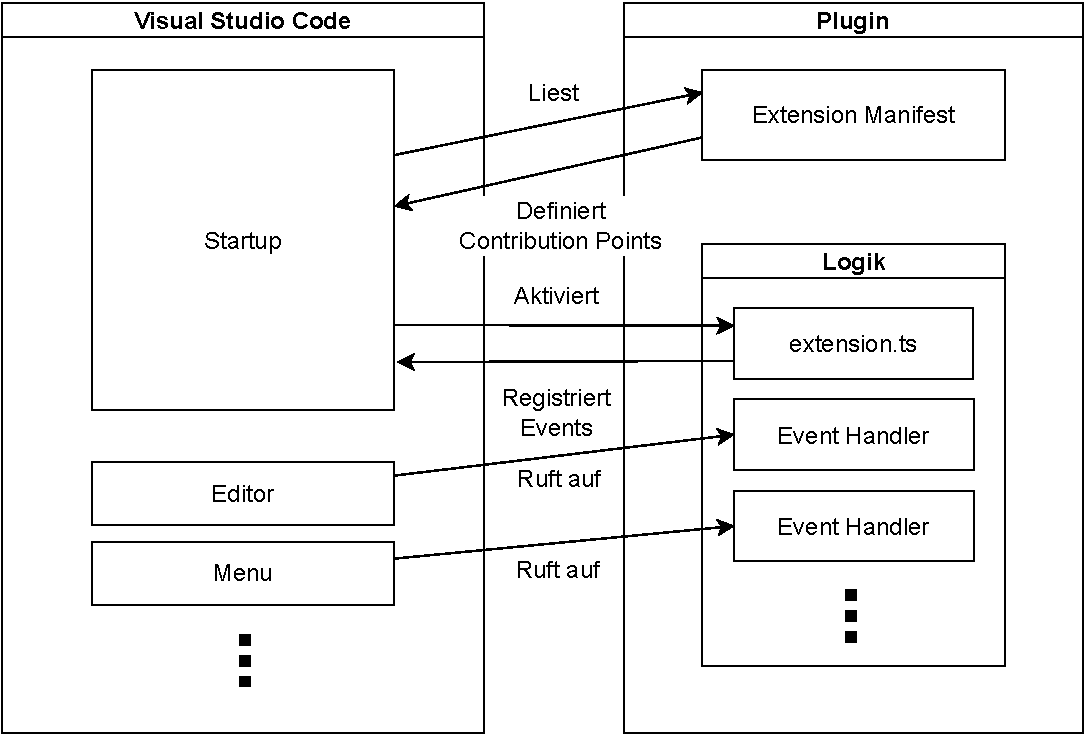
\includegraphics[width=.95\textwidth]{diagram_VSCodeExtensionArchitecture}}
    \caption{Übersicht über den Ablauf eines VS Code Plugins.}
    \label{fig:diagram_VSCodeExtensionArchitecture}
  \end{figure}   

\subsection{IntelliJ IDEA}

Der Aufbau der Plugin Architektur wirkt bei IntelliJ im ersten Moment genau
gleich wie bei Visual Studio Code. Es gibt nämlich auch hier gibt
es ein Plugin Configuration File, sowie ein Modul mit API Schnittstellen.
Der große Unterschied liegt allerdings in der Funktionsweise und der Interaktion
mit den Plugins und der Art wie der auszuführende Code angegeben wird.
\subsubsection{Plugin Configuration File}
  Die Konfiguration eines Plugins liegt in der \enquote{plugin.xml} Datei und
  beinhaltet, equivalent zum Extension Manifest in VS Code, alle für das Plugin
  notwendigen Meta-Informationen. So können auch hier Werte wie der Name,
  eine Beschreibung, die aktuelle Versionsnummer und so weiter angegeben werden.
  Für die Funktionen die das Plugin mitbringt gibt es Actions, Extension Points
  und Listener. Hier ist anzumerken, dass es sich sowohl bei den Extension Points,
  als auch den Listenern, immer direkt um eine Zuordnung eines Interfaces
  (meist definiert von IntelliJ) zu einer Implementierung (definiert durch das Plugin)
  handelt. Weiters ist es nicht nötig einen speziellen Aktivierungszeitpunkt
  festzulegen, da die zuordnung der auszuführenden Klassen sowieso durch 
  die Konfigurationsdatei festgelegt wird. Eine Besonderheit an IntelliJ ist,
  dass Plugins auch eigene Extension Points definieren können, um weiteren Plugins
  das erweitern des ursprünglichen Plugins zu erlauben.
\subsubsection{IntelliJ Platform SDK}
  Die API für IntelliJ Plugins ist in mehreren Paketen des IntelliJ 
  Platform SDK enthalten. Diese API enthält auch die unterschiedlichen
  Interfaces, welche dann in Form von Extension Points oder Listenern implementiert
  werden können. 
\subsubsection{Ablauf}
  IntelliJ analysiert zuerst das Plugin Configuration File.
  Je nachdem welche Funktionalität vom Plugin angeboten wird, werden
  von IntelliJ automatisch die entsprechenden Event Handler 
  auf die unterschiedlichen Extension Points registriert. 
  Die registrierten Handler werden dann während der Ausführung und Verwendung
  von IntelliJ aufgerufen und können so beliebigen Code ausführen.
  Siehe Abbildung \ref{fig:diagram_IntelliJExtensionArchitecture}.
  \begin{figure}
    \centering
    \fbox{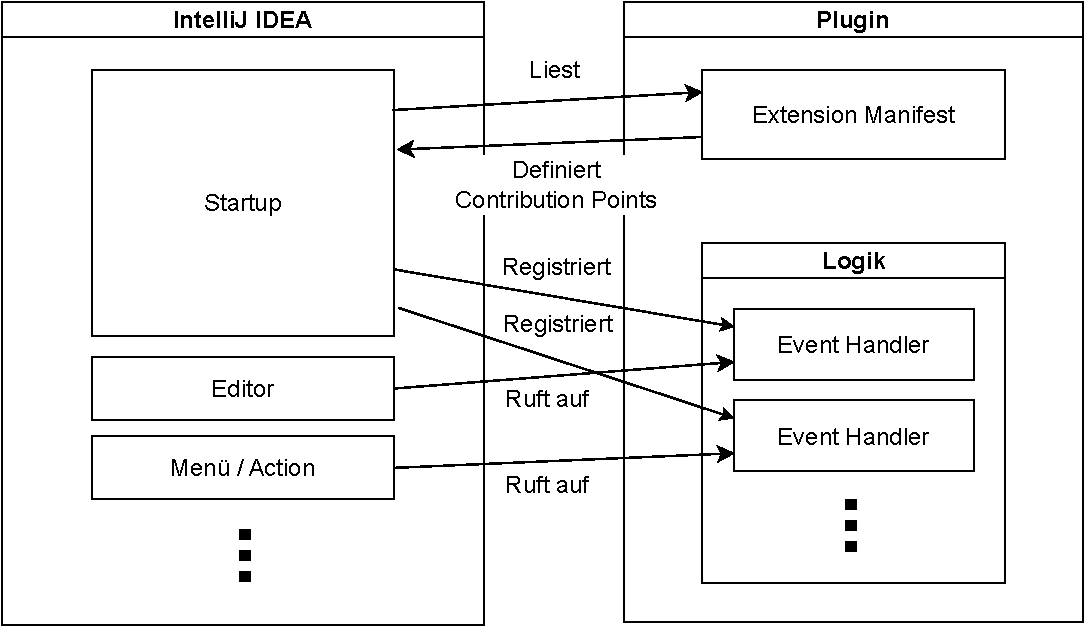
\includegraphics[width=.95\textwidth]{IntelliJExtensionArchitecture}}
    \caption{Übersicht über den Ablauf eines IntelliJ.}
    \label{fig:diagram_IntelliJExtensionArchitecture}
  \end{figure}   

\section{Funktionalität der Plugin API}
\label{sec:FunktionalitätDerPluginAPI}

\subsection{Visual Studio Code}

\subsection{IntelliJ IDEA}

\subsection{IntelliJ Flora Plugins}

In der Plugin Dokumentation von JetBrains wird zu Beginn 
empfohlen sich noch einmal gründlich zu überlegen, ob man 
für die von einem gewünschte Funktionalität wirklich ein 
vollwertiges Plugin benötigt. Häufig kommt es nämlich vor, 
dass nur bestimmte kleine Tasks innerhalb des IDEs 
automatisiert werden sollen \cite{IntelliJSDKDocumentation}. Hierfür schlägt JetBrains 
einige leichtgewichtige Alternativen vor. Eine nennenswerte 
Alternative ist das „Flora Plugin“ für das IntelliJ IDEA. 

Flora kann über die Einstellungen des IntelliJ IDEA 
im Abschnitt „Plugins“ installiert werden.

% //TODO rework screenshots

\begin{figure}
    \centering
    \fbox{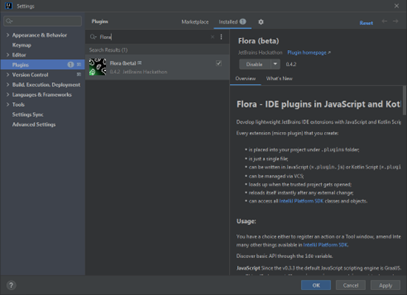
\includegraphics[width=.95\textwidth]{flora_plugin}}
    \caption{Flora Plugin im IntelliJ Plugin Marketplace.}
    \label{fig:FloraPlugin}
\end{figure}    
 
Das Plugin sucht dann in den geöffneten Projektverzeichnissen
nach ausführbaren JavaScript oder Kotlin Script „micro plugin“ 
Dateien. Diese müssen sich in einem Ordner namens „.plugins“ 
befinden und auf „.plugin.js“ oder „.plugin.kts“ enden \cite{FloraPluginMarketplace}.
Innerhalb diese Plugin Dateien kann über die Variable „ide“ auf 
die angebotene Schnittstelle zugegriffen werden. Diese erlaubt 
es unter anderem Actions, Keyboard Shortcuts, Services und 
ToolWindows zu erstellen.

\begin{figure}
    \centering
    \fbox{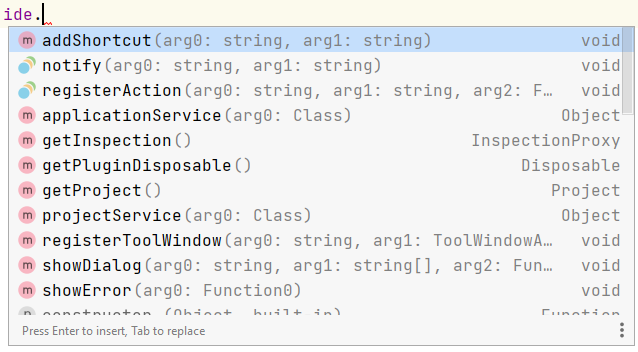
\includegraphics[width=.95\textwidth]{flora_codeCompletion}}
    \caption{Übersicht über die API des Flora Plugins.}
    \label{fig:FloraPluginAPI}
\end{figure}    
 
Flora Plugins bieten sich vor allem dann an, wenn eine projektspezifische 
Aufgabe automatisiert werden soll. Hier sind vor Allem die 
Leichtgewichtigkeit der Plugins und die Schnelle, mit der ein 
einfaches Plugin entwickelt werden kann, von großem Vorteil. 
Weiters spricht für diesen Anwendungsfall, dass der Plugin Code 
direkt im Projektordner abgelegt wird und somit auch in einem Version 
Control System wie Git mit abgelegt werden kann.
